\documentclass[12pt]{article}
\usepackage{amssymb,mathtools}
\usepackage[margin=1in]{geometry}
\usepackage{fancyhdr}
\usepackage{circuitikz}
\usepackage{graphicx}
\graphicspath{ {./Figures/} }
\usepackage{amsmath}
\usepackage{ragged2e}
\usepackage{subcaption} 
\usepackage{float}
\usepackage{cancel}
\usepackage{siunitx}
\pagestyle{fancy}
\usepackage[shortlabels]{enumitem}
\usepackage{mathtools}
\newcommand*{\permcomb}[4][0mu]{{{}^{#3}\mkern#1#2_{#4}}}
\newcommand*{\Comb}[2]{{}^{#1}C_{#2}}%
\DeclarePairedDelimiter\ceil{\lceil}{\rceil}
\DeclarePairedDelimiter\floor{\lfloor}{\rfloor}
\setlength{\headheight}{15 pt}
\lhead{Georgy Antonov}
\chead{HW 6}
\rhead{Neural Dynamics}

\begin{document}\noindent


\noindent\textbf{Question 1. Linear Dynamical System.}
\begin{enumerate}
\item[]We have the following linear dynamical system 
\[
    \dot{\mathbf{x}}(t) = \mathbf{Ax}(t) + \mathbf{s}(t)
\]
where
$$A = \begin{pmatrix}
    -0.5 & -0.5 & 0\\
    -0.5 & -0.5 & 0\\
        0 &    0 & 2
\end{pmatrix}$$
\item[1.1] Assuming $\mathbf{s}(t)=0$, we need to compute and sketch the solutions for the initial conditions
\[
    \mathbf{x}_{0,1} = \begin{pmatrix} 1\\ 1\\ 0 \end{pmatrix}, \quad 
    \mathbf{x}_{0,2} = \begin{pmatrix} 1\\ 0\\ 0 \end{pmatrix}, \quad
    \mathbf{x}_{0,3} = \begin{pmatrix} 0\\ 1\\ 0 \end{pmatrix}, \quad
    \mathbf{x}_{0,4} = \begin{pmatrix} 0\\ 0\\ 10^{-6} \end{pmatrix}
\]

Note that the initial value problem has a solution of the form
\[
    \mathbf{x}(t) = e^{\mathbf{A}t} \mathbf{x}_{0}
\]
For non-singular $\mathbf{A}$, we can rewrite it as follows
$$\mathbf{x}(t)=\mathbf{Q}e^{\mathbf{\Lambda} t}\mathbf{Q}^{-1}\mathbf{x}_{0}$$
where $\mathbf{Q}$ is a matrix of eigenvectors and $\mathbf \Lambda$ is a daigonal matrix with non-zero entries representing corresponding eigenvalues.
To solve this, we have to first find the eigenvalues and eigenvectors of $\mathbf{A}$. 
Hence, we start by solving the characteristic equation
\[
    \text{det}\left(A - I\lambda\right) = 0
\]
\[
\begin{vmatrix} -0.5 - \lambda & -0.5 & 0\\ -0.5 & -0.5 - \lambda & 0\\ 0 & 0 & 2-\lambda \end{vmatrix}
    = 0 \quad \iff \quad -\lambda^{3} + \lambda^{2} + 2\lambda = 0
\]
We find that $\mathbf{A}$ has three distinct eigenvalues, namely, $\lambda_{1}=0, \, \lambda_{2}=2, \, \lambda_{3}=-1$, with 
the corresponding eigenvectors
\[
\mathbf{v}_{1}=\begin{pmatrix} -1\\ 1\\ 0 \end{pmatrix}, \quad \mathbf{v}_{2}=\begin{pmatrix} 0\\ 0\\ 1 \end{pmatrix}, \quad \mathbf{v}_{3}=\begin{pmatrix} 1\\ 1\\ 0 \end{pmatrix}
\]
Now, we have
\begin{align*}
    \mathbf{Q}=\begin{pmatrix} -1 & 0 & 1\\ 1 & 0 & 1\\ 0 & 1 & 0 \end{pmatrix}, & \quad \mathbf{\Lambda} = \begin{pmatrix} 0 & 0 & 0\\ 0 & 2 & 0\\ 0 & 0 & -1 \end{pmatrix}
\end{align*}
and we can thus write our solution as follows
\begin{align*}
\mathbf{x}(t) &= \begin{pmatrix} -1 & 0 & 1\\ 1 & 0 & 1\\ 0 & 1 & 0 \end{pmatrix}
                \begin{pmatrix} 1 & 0 & 0\\ 0 & e^{2t} & 0\\ 0 & 0 & e^{-t} \end{pmatrix}
                \begin{pmatrix} -1 & 0 & 1\\ 1 & 0 & 1\\ 0 & 1 & 0\\ \end{pmatrix}^{\!-1}\mathbf{x}_{0}\\
\implies \mathbf{x}(t) &= \begin{pmatrix} -1 & 0 & 1\\ 1 & 0 & 1\\ 0 & 1 & 0 \end{pmatrix} \begin{pmatrix} -0.5 & 0.5 & 0\\ 0 & 0 & e^{2t}\\ 0.5e^{-t} & 0 & 0\\ \end{pmatrix}\mathbf{x}_{0}\\
\implies \mathbf{x}(t) &= \begin{pmatrix} 0.5+0.5e^{-t} & -0.5 & 0\\ -0.5+0.5e^{-t} & 0.5 & 0\\ 0 & 0 & e^{2t}\end{pmatrix}\mathbf{x}_{0}
\end{align*}
And in a non-matrix form this becomes 
\[
\mathbf{x}(t)=\begin{pmatrix} (0.5 + 0.5e^{-t})x_{1} - 0.5x_{2}\\ (-0.5 + 0.5e^{-t})x_{1} + 0.5x_{2}\\ e^{2t}x_{3}\end{pmatrix}
\]
Finally, for the aforementioned initial conditions we have
\begin{align*}
\mathbf{x}_{0,1}(t)&=\begin{pmatrix} 0.5+0.5e^{-t} & -0.5 & 0\\ -0.5+0.5e^{-t} & 0.5 & 0\\ 0 & 0 & e^{2t}\end{pmatrix} \begin{pmatrix} 1\\ 1\\ 0 \end{pmatrix} = \begin{pmatrix} 0.5e^{-t}\\ 0.5e^{-t}\\ 0 \end{pmatrix}\\
\mathbf{x}_{0,2}(t)&=\begin{pmatrix} 0.5+0.5e^{-t} & -0.5 & 0\\ -0.5+0.5e^{-t} & 0.5 & 0\\ 0 & 0 & e^{2t}\end{pmatrix} \begin{pmatrix} 1\\ 0\\ 0 \end{pmatrix} = \begin{pmatrix} 0.5+0.5e^{-t}\\ -0.5+0.5e^{-t}\\ 0 \end{pmatrix}\\
\mathbf{x}_{0,3}(t)&=\begin{pmatrix} 0.5+0.5e^{-t} & -0.5 & 0\\ -0.5+0.5e^{-t} & 0.5 & 0\\ 0 & 0 & e^{2t}\end{pmatrix} \begin{pmatrix} 0\\ 1\\ 0 \end{pmatrix} = \begin{pmatrix} -0.5\\ 0.5\\ 0 \end{pmatrix}\\
\mathbf{x}_{0,4}(t)&=\begin{pmatrix} 0.5+0.5e^{-t} & -0.5 & 0\\ -0.5+0.5e^{-t} & 0.5 & 0\\ 0 & 0 & e^{2t}\end{pmatrix} \begin{pmatrix} 0\\ 0\\ 10^{-6} \end{pmatrix} = \begin{pmatrix} 0\\ 0\\ 10^{-6}e^{t} \end{pmatrix}
\end{align*}
And the phase diagrams for these initial conditions appear in Figures 1-4.
\begin{figure}[h!]
    \centering
    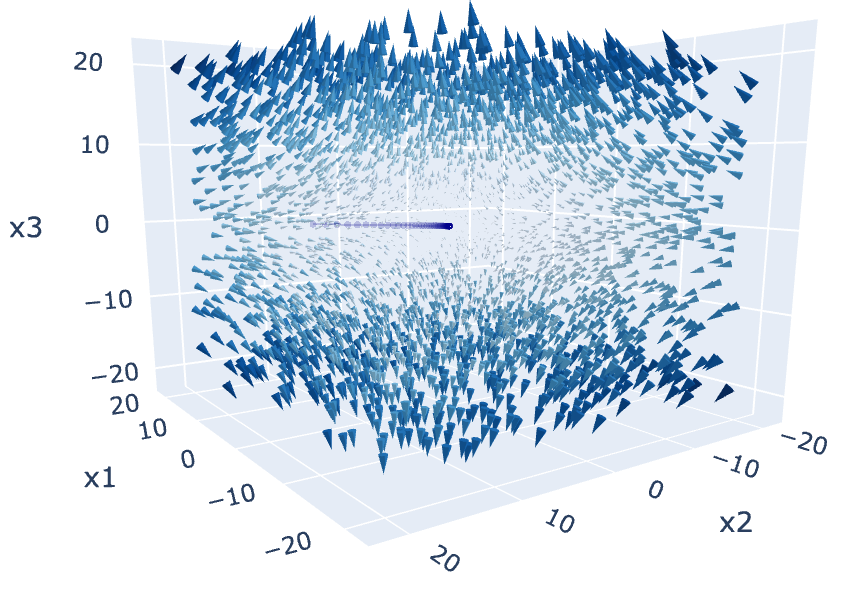
\includegraphics[width=1\textwidth]{Figures/1.png}
    \caption{3D dynamics of $\mathbf{x}(t)$ following the initial condition $\mathbf{x}_{0,1}$ for $t \in [-3, 3]$.}
\end{figure}
\begin{figure}[h!]
    \centering
    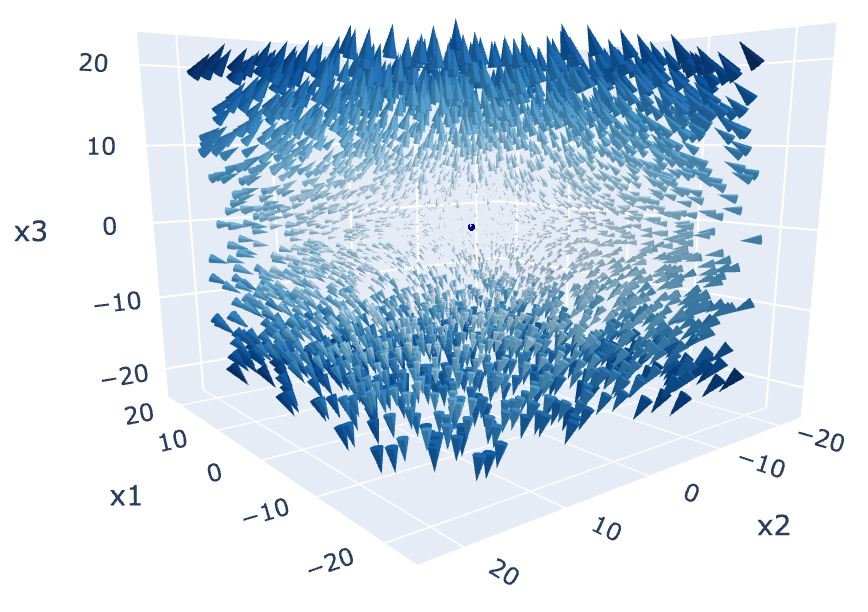
\includegraphics[width=1\textwidth]{Figures/2.png}
    \caption{3D dynamics of $\mathbf{x}(t)$ following the initial condition $\mathbf{x}_{0,2}$.}
\end{figure}
\begin{figure}[h!]
    \centering
    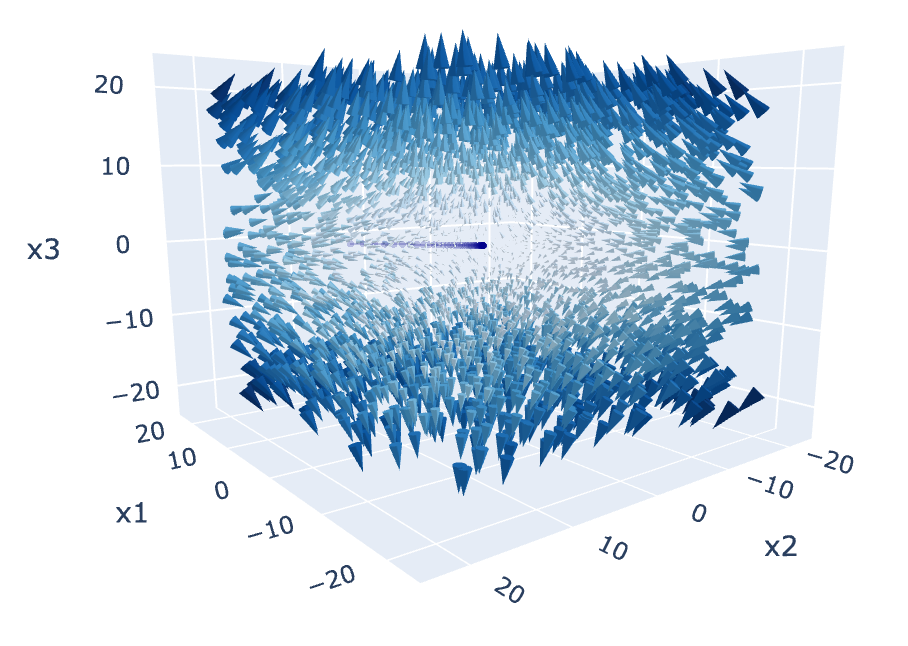
\includegraphics[width=1\textwidth]{Figures/3.png}
    \caption{3D dynamics of $\mathbf{x}(t)$ following the initial condition $\mathbf{x}_{0,3}$ for $t \in [-3, 3]$.}
\end{figure}
\begin{figure}[h!]
    \centering
    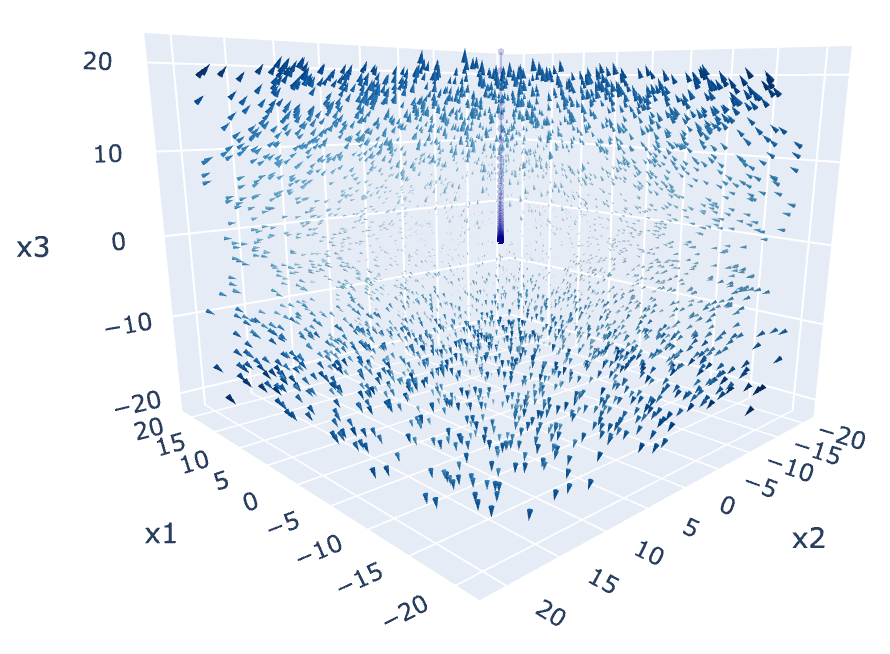
\includegraphics[width=1\textwidth]{Figures/4.png}
    \caption{3D dynamics of $\mathbf{x}(t)$ following the initial condition $\mathbf{x}_{0,4}$ for $t \in [-17, 17]$.}
\end{figure}
\item[1.2] The eigenvalues and eigenvectors of $\mathbf{A}$ were computed in 1.1. Eigenvalue sign tells us about
the direction and speed of the dynamics evolution, and the eigenvectors tell us in which direction the flow will be linear, i.e. only 
affected by the dynamics matrix as a scalar multiplication. 
\item[1.3] The projections of $\mathbf{f}(x)=\mathbf{Ax}$ appear in Figures 5-7.
\begin{figure}[h!]
    \centering
    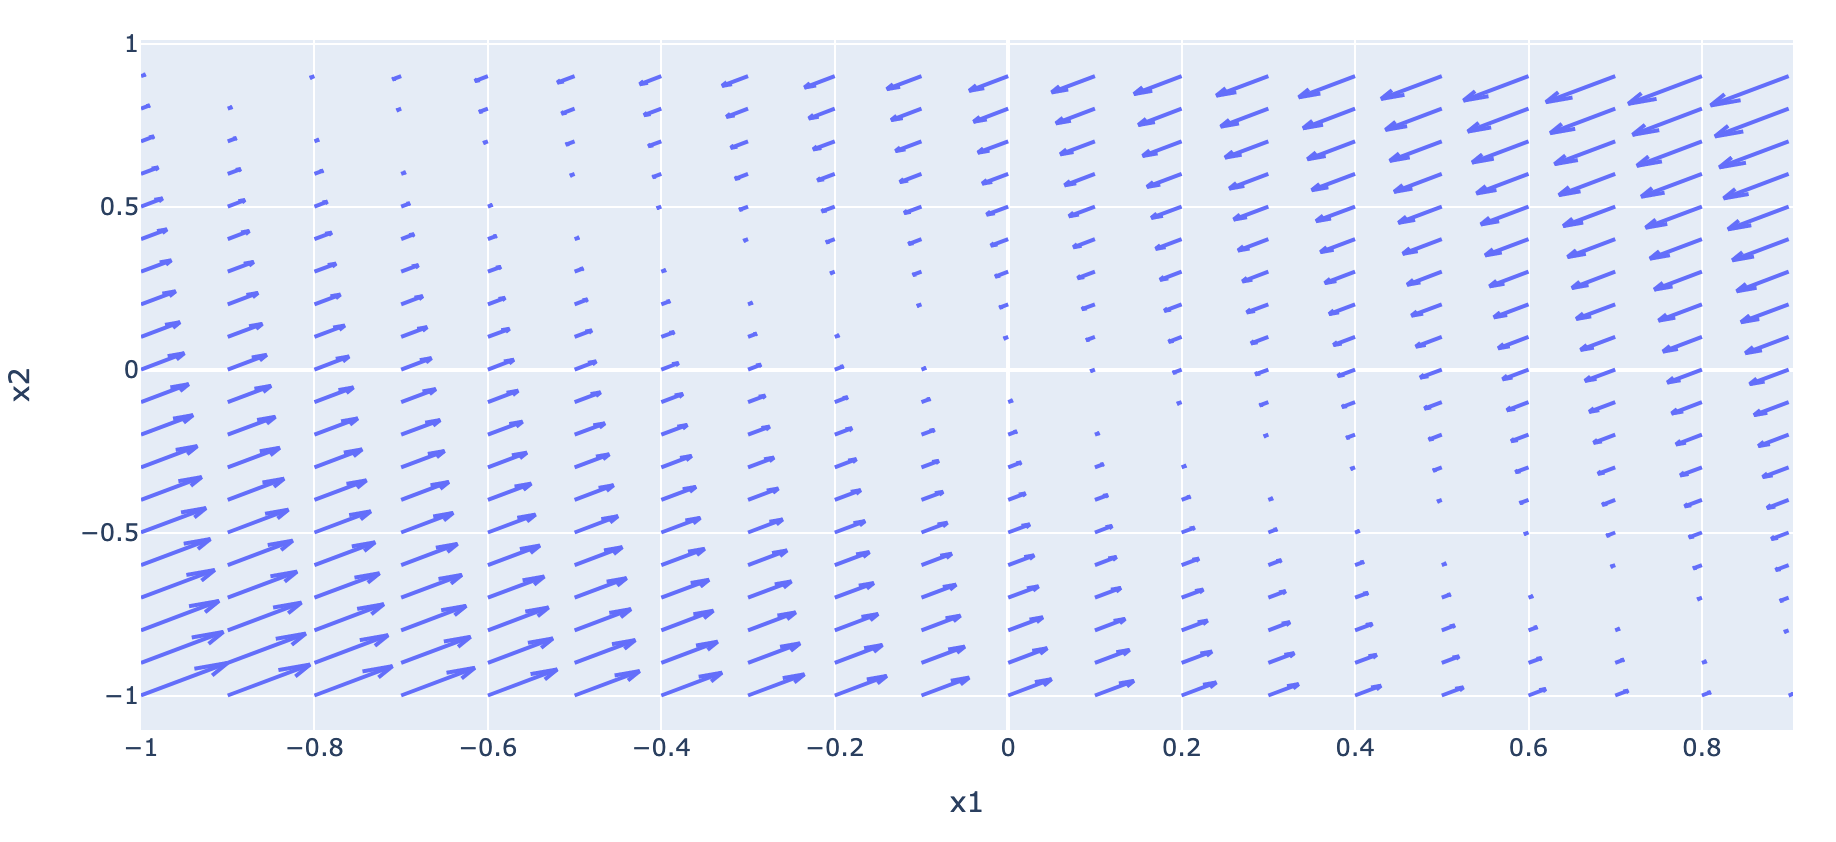
\includegraphics[width=1\textwidth]{Figures/x1x2.png}
    \caption{Projection of $\mathbf{f}(x)=\mathbf{Ax}$ onto a plane defined by $x_{3}=0$.}
\end{figure} 
\begin{figure}[h!]
    \centering
    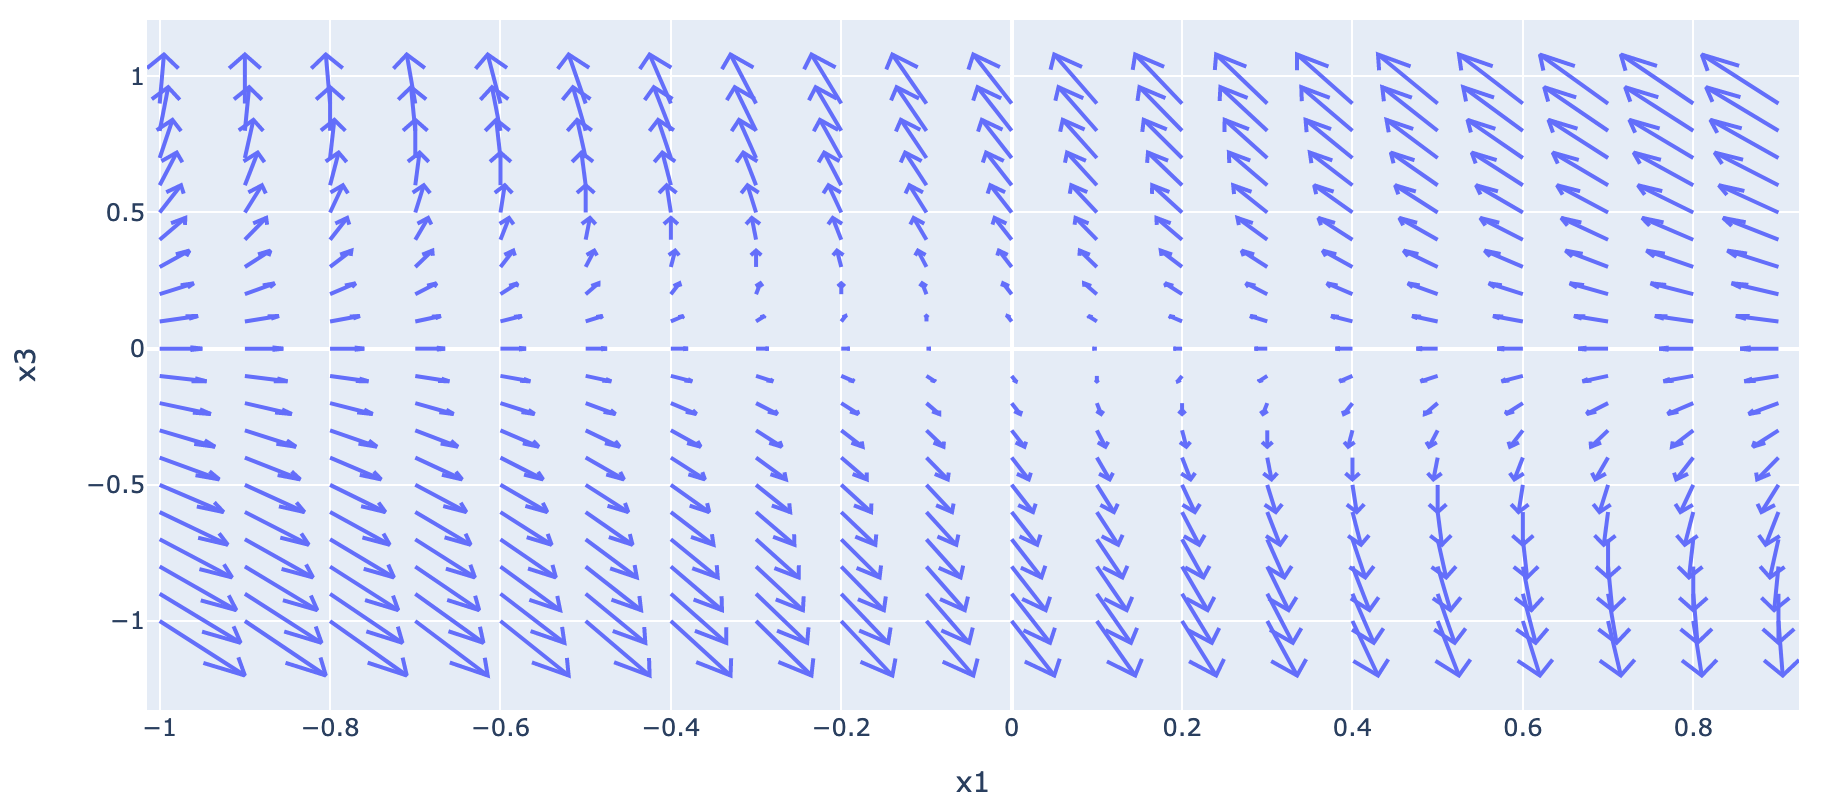
\includegraphics[width=1\textwidth]{Figures/x1x3.png}
    \caption{Projection of $\mathbf{f}(x)=\mathbf{Ax}$ onto a plane defined by $x_{2}=0$.}
\end{figure} 
\begin{figure}[h!]
    \centering
    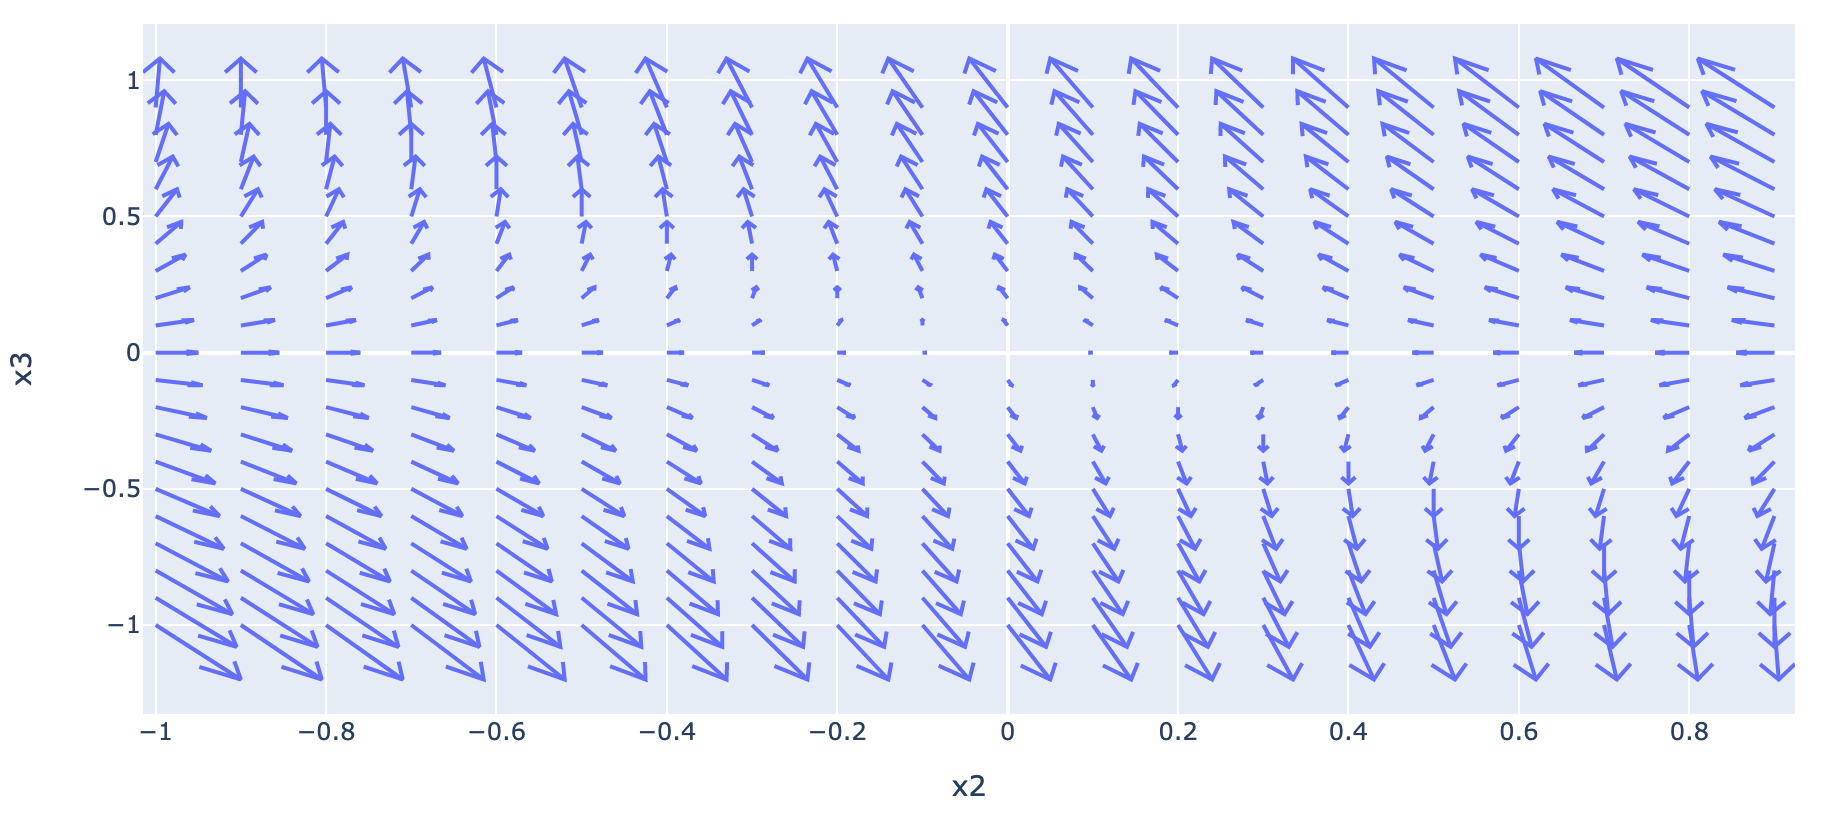
\includegraphics[width=1\textwidth]{Figures/x2x3.png}
    \caption{Projection of $\mathbf{f}(x)=\mathbf{Ax}$ onto a plane defined by $x_{1}=0$.}
\end{figure} 
The dynamics observed in Figure 5 can be explained using the fact that the eigenvalue associated with eigenvector $\mathbf{v}_{1}$ is zero.
Therefore, we see an invariant manifold along the direction of this eigenvector, with particles attracted towards it. As for Figures 6 and 7, there 
is a saddle point at $(0, 0)$, for there is one stable and one unstable direction.
\item[1.4] Now we want to project the vector field of the dynamics onto the subspace defined by basis
\[
\mathbf{e}_{1}=\frac{1}{\sqrt{2}}\begin{pmatrix}1\\ -1\\ 0\end{pmatrix}, \quad \mathbf{e}_{2}=\begin{pmatrix}0\\ 0\\ 1\end{pmatrix}
\] 
Recall the formula for projecting vector $\mathbf{x}$ onto a line spanned by vector $\mathbf{u}$
\[
    \text{proj}_{\mathbf{u}}(\mathbf{x}) = \frac{\mathbf{u} \cdot \mathbf{x}}{\|\mathbf{u}\|}\mathbf{u}
\]
Therefore, to project vector $\mathbf{x}$ onto a subspace V spanned by $\mathbf{e}_{1}$ and $\mathbf{e}_{2}$, we need to do the following
\[
    \text{proj}_{V}(\mathbf{x}) = \frac{\mathbf{e}_{1} \cdot \mathbf{x}}{\|\mathbf{e}_{1}\|}\mathbf{e}_{1} + \frac{\mathbf{e}_{2} \cdot \mathbf{x}}{\|\mathbf{e}_{2}\|}\mathbf{e}_{2}
\]
And since $\mathbf{e}_{1}$ and $\mathbf{e}_{2}$ form the basis, we know they are unit vectors, and hence we are left with
\[
    \text{proj}_{V}(\mathbf{x}) = \left(\mathbf{e}_{1} \cdot \mathbf{x}\right)\mathbf{e}_{1} + \left(\mathbf{e}_{2} \cdot \mathbf{x}\right)\mathbf{e}_{2}
\]
\end{enumerate}
\end{document}
